\newcommand{\xbr}{\left(x\right)}
\newcommand{\br}[1]{\left(#1\right)}
\newcommand{\abs}[1]{\left|#1\right|}

\chapter{The model}

\section{Problem statement}

The system under consideration consists of two 1D s-type superconducting wires connected with a tunnel junction. There is a strong spin-orbit coupling assumed to be present and external magnetic field is applied in the direction perpendicular to the wire. The Hamiltonianm of the bulk of each wire, written in the Bogoliubov-de Gennes formalism, is similar to the ones presented in \cite{Oreg_2010} and \cite{Lutchyn_2010}:

\begin{gather}
	\mathcal{H}
	=
	\int dy ~
	\Psi^\dagger
	\br{y}
	H
	\Psi
	\br{y}
	\
	~~~~
	\Psi
%	\left(x\right)
	=
	\begin{pmatrix}
		\psi_\uparrow
		\\
		\psi_\downarrow
		\\
		\psi_\downarrow^\dagger
		\\
		-\psi_\uparrow^\dagger
	\end{pmatrix}
	\\
	\label{bulk_Hamiltonian}
	H
	=
	\br{
		\frac{p^2}{2m}
		-\mu_0
	}\tau_z
	+
	u p \sigma_z \tau_z
	+
	B\sigma_x	
	+
	\Delta\tau_\phi
\end{gather}

Here $ \sigma_i $ and $ \tau_i $ are Pauli matrices in spin and particle-hole subspaces respectfully, $ \tau_\phi = \tau_x \cos\phi - \tau_y \sin\phi$, with $ \phi $ being a superconducting phase, $ \mu_0 $ is a chemical potential, $ B $ is an external magnetic field, $ \Delta $ is the absolute value of superconducting order parameter and $ u $ is spin-orbit coupling constant with the dimension of velocity. The wire is being aligned along the y-axis, while the direction of the magnetic field coincides with x-axis. Note, that only one component of spin-orbit is nonzero due to 1D nature of the problem.

The tunnel junction is introduced  by applying an external electrical field. It's potential profile $U\br{y}  $ is presented at figure \ref{fig:chemandextpotentials}(a). Inside each wire the potential is assumed to be homogeneous, thought it's value can be different to the right and to the left of the junction. The junction itself is modeled by a sharp pike of the potential.
 
To take this into account one should include an additional term $ U \br{y}\tau_z $ in (\ref{bulk_Hamiltonian}). However this term can be combined with the second term of  by (\ref{bulk_Hamiltonian}) by introducing an effective chemical potential $ \mu \br{y} = \mu_0 - U\br{y}  $ (see figure \ref{fig:chemandextpotentials}(b)). From now on all presence of  the external field will be hidden in $ \mu\br{y} $.

The superconducting phase $ \phi $ in left and right wires, $ \phi_L $ and $ \phi_R $, can also be different. The phase inside the barrier is assumed to be a continuous monotonous function going from $ \phi_L $ to $ \phi_R $. The exact shape of that function is not important, as $ \mu\br{y} \gg \Delta$ inside the   
barrier.



\begin{figure}[H]
	\centering
	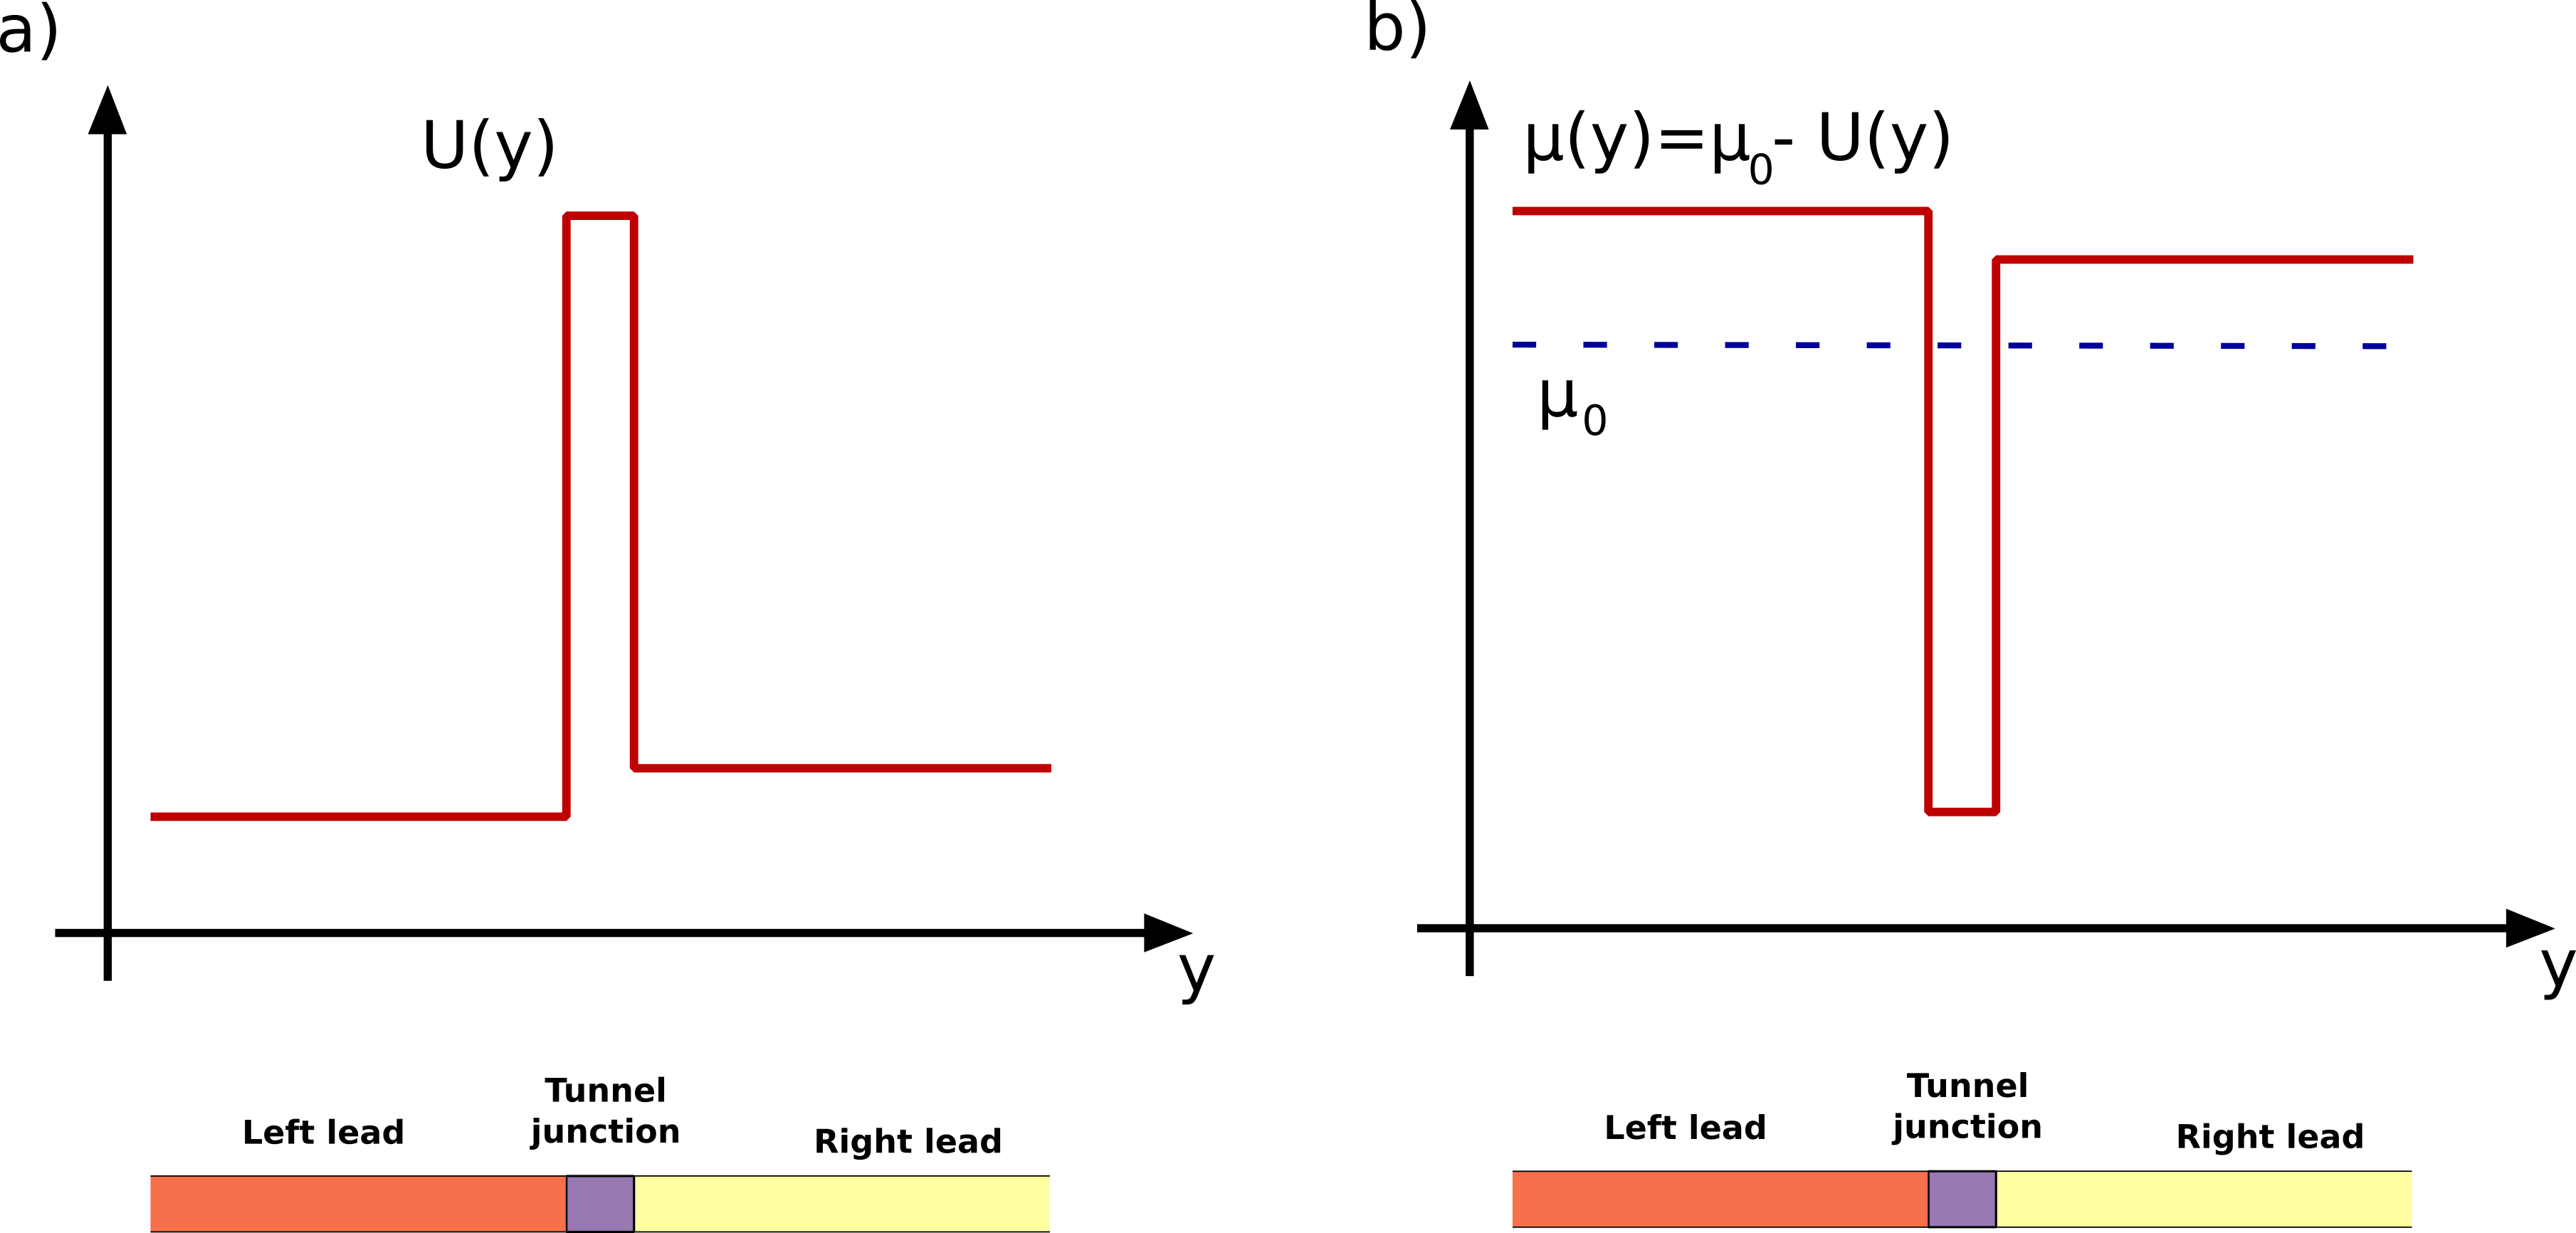
\includegraphics[width=0.8\linewidth]{images/chem_and_ext_potentials}
	\caption{(a) y-profile of external electrical field.  (b) y-profile of effective chemical potential}
	\label{fig:chemandextpotentials}
\end{figure}


Finally, the BdG Hamiltonian for the model reads:

\begin{equation}
\label{full_hamiltonian}
H
=
\br{
	\frac{p^2}{2m}
	-\mu\br{y}
}\tau_z
+
u p \sigma_z \tau_z
+
B\sigma_x	
+
\Delta\tau_{\phi\br{y}}
\end{equation}

with

\begin{equation}
\label{full_hamiltonian_suppl}
	\mu\br{y}
	=
	\begin{cases}
		\mu_L,~~~  -\frac{L}{2}<y\\
		\mu_b,~~ -\frac{L}{2} <y <\frac{L}{2}\\
		\mu_R, ~~~~ \frac{L}{2}< y  
	\end{cases}
	~~~~~~~~
	\phi\br{y}
	=
	\begin{cases}
		\phi_L,&~~~  -\frac{L}{2}<y\\
		\phi_R
		\frac{\frac{L}{2}+y}{L}
		+
		\phi_L
		\frac{\frac{L}{2}-y}{L},
		&~~ -\frac{L}{2} <y <\frac{L}{2}\\
		\phi_R, &~~~~ \frac{L}{2}< y 
	\end{cases}
\end{equation}
with $ L $ being the size of the junction. Note, that the parameters $ B $, $ u $, $ \Delta $ and $ m $ are taken to be constant within all the system.
 
  This setup is close to the one of the models  considered by Oreg et al. in \cite{Oreg_2010} ("\textit{Spatially varying $ \mu $}" section). The difference is in the profile of $ \mu\br{y} $ -- in \cite{Oreg_2010}  there is a step in effective chemical potential, while here this function possesses a well.  
  
 In \cite{Oreg_2010} it's also discussed that the Majorana fermion appear at the inhomogeneity if the relation $ B-\sqrt{\mu^2+\Delta^2} $ is greater than zero at one side of the step in $ \mu\br{y} $ and lesser than zero at another side of it. As will be shown further, this is also relevant to the  system presented here. Note, that if $ B > \left|\Delta\right| $ this condition can always be satisfied by choosing appropriate $ \mu_L $ and $ \mu_R $. 
 
 The model, described by (\ref{full_hamiltonian}) and (\ref{full_hamiltonian_suppl}) possesses a big number of external parameters. Different areas in this parameter space require different approaches and sometimes lead to completely different physics. Here the certain experimentally reasonable constraints are assumed:
 
 \begin{gather}
 \label{constraints}
 	\mu_L,\mu_R \ll B \sim \Delta \ll mu^2\ll \left|\mu_b\right|
 \end{gather} 

  The experimental justification of this choice is given in the section \textbf{SECTION ABOUT REALIZATION}, while call for it from theoretical point of view will arise further in this chapter.
  


\section{The dispersion of a homogeneous wire}

Before discussing the properties of the junction it's necessary to consider a dispersion of a homogeneous wire modeled with the Hamiltonian (\ref{bulk_Hamiltonian}). Although this can be done exactly, it's instructive to obtain this dependence step by step, starting with a simpler model and adding new terms until the Hamiltonian (\ref{bulk_Hamiltonian}) is restored.

The starting point is the Hamiltonian consisting only of kinetic energy and chemical potential terms: $ H =\frac{ p^2}{2m} - \mu$. It has simple parabolic dispersion presented at fig. \ref{fig:spectrum}(a). When the spin is introduced and spin-orbit coupling term $ up\sigma_z $ is added, the parabola splits in two (fig. \ref{fig:spectrum}(b)), each one corresponding to it's own z-protection of the spin. After introducing a magnetic field with $ B\sigma_x $ term, the gap at the intersection opens (fig. \ref{fig:spectrum}(c)). The next step is introducing the BdG formalism, by adding the multiplier $ \tau_z $ elsewhere except for magnetic field term:  $ 	H = \br{\frac{p^2}{2m} 	-\mu_0 }\tau_z +u p \sigma_z \tau_z + B\sigma_x	 $. This procedure doubles the spectra in a way that each eigenvector with energy $ E $ obtains a partner eigenvector with energy $ -E $, so additional two energy branches appear, being a mirror reflection of  initial dispersion. This is presented at fig. \ref{fig:spectrum}(d), with the dashed lines being BdG partners. The last step is adding the superconducting term $ \Delta\tau_\phi $, which opens the gap where the dashed and the solid lines are intersected (fig. \ref{fig:spectrum}(f)).

As was mentioned before, the dispersion can be found explicitly. As was pointed in \cite{Oreg_2010}, it can be done by squiring the Hamiltonian (\ref{bulk_Hamiltonian}) twice and solving a resulting biquadratic equation, leading to:


\begin{equation}
E^2_{1,2}\br{p}
=
B^2
+
\Delta^2
+
\xi_p^2
+
\br{up}^2
\pm	
2\sqrt{
	B^2 \Delta^2
	+
	B^2\xi_p^2
	+
	\br{up}^2\xi_p^2
}
\end{equation}

with $ \xi_p =\frac{p^2}{2m}-\mu$. This dependence, presented at fig. \ref{fig:spectrum}(f), has two positive and two negative branches, as any BdG dispersion with electron-hole symmetry does. It further discussion only positive branches are considered, if opposite is not mentioned.

\begin{figure}[H]
	\centering
	\includegraphics[width=\linewidth]{images/spectrum}
	\caption{The dispersion of different Hamiltonians:
		 a)  mere kinetic energy and chemical potential: $ H =\frac{ p^2}{2m} - \mu ~~~$
		 b) spin-orbit coupling added: $ 	H = \frac{p^2}{2m}-\mu_0 + u p \sigma_z ~~~$
		 c) magnetic field added: $ 	H = \frac{p^2}{2m} 	-\mu_0  +u p \sigma_z  + B\sigma_x ~~~~~$
		 d) BdG formalism introduced: $ 	H = \br{\frac{p^2}{2m} 	-\mu_0 }\tau_z +u p \sigma_z \tau_z + B\sigma_x	~~~ $
		 e) complete Hamiltonian of homogeneous wire: $ 	H = \br{\frac{p^2}{2m} 	-\mu_0 }\tau_z +u p \sigma_z \tau_z + B\sigma_x	+ \Delta\tau_\phi $.
		 The parameters of the Hamiltonians for plotting are: $ B=0.2 $, $ \Delta=0.3 $, $ u=0.9 $, $ m = 1 $, $ \mu = 0.11 $ 
 }
	\label{fig:spectrum}
\end{figure}

If the constrains (\ref{constraints}) are assumed, the lower branch of this spectra has three minima: one of them is at $ p=0 $ exactly, and two another are at $ p = \pm 2mu $ in the leading order. The last two are not very interesting -- the energy there is approximately equal to $ \Delta $, as it should be due to perturbative introduction of superconducting term. On the contrary, the minimum at $ p=0 $, which is given by\cite{Oreg_2010}:

\begin{gather}
	E_2\br{0}=\abs{g},~~~~g = B^2 -\sqrt{\Delta^2+\mu^2}
\end{gather}

is the most important peculiarity of the spectrum. First, as $\mu\ll B \sim \Delta $, it's the true gap of the spectrum as $  \abs{B^2 -\sqrt{\Delta^2+\mu^2}} \approx  \abs{B-\Delta -\frac{\mu^2}{2\Delta}}\ll\Delta$. Second, the  sign of  $ g $ defines where the wire can or cannot host the Majorana state near some inhomogeneity. Here it's useful to introduce the terminology: if $ g>0 $ the wire is called "toplogical", otherwise it's called "trivial". In \cite{Oreg_2010} and \cite{Lutchyn_2010} it was derived, that the contact of trivial and topological wire hosts a Majorana state. It can also be shown (see section \textbf{ENTER SECTION}), that this state is present on the end of a topological wire and isn't there for a trivial one.


\section{Wavefunctions of a homogeneous wire}

Though the wavefunctions of (\ref{bulk_Hamiltonian}) can be found explicitly, their form is enough complicated to stall any further analysis. Here it's reasonable  to recall that due to constraints (\ref{constraints}) the spin-orbit energy $ mu^2 $ is the biggest energy parameter for homogeneous wire (the parameter $ \mu_b $ appears only when barrier is introduced). At first it seems that for the leading approximation it's enough to use the Hamiltonian: $ 	H
=
\br{
\frac{p^2}{2m}
+
u p \sigma_z }\tau_z $. However the spectrum of this Hamiltonian is ungapped, and all it's solutions will have the form of running waves. To find any decaying states, the gap in the spectrum is required, so it's necessary to keep the superconducting term in the Hamiltonian and solve the equation:
\begin{gather}
\left[
\br{
\frac{p^2}{2m}
+
u p \sigma_z} \tau_z
+
\Delta
\tau_\phi
\right]
\psi
=
0
\end{gather}

The zero in the l.h.s. is justified by the fact, that all the Majorana physics occur at the energies if the order of $ g $, so the term $ E\psi $ doesn't contribute to the leading order.
